\documentclass{article}
\usepackage[italian]{babel}  
\usepackage[utf8]{inputenc}
\usepackage[T1]{fontenc}
\usepackage{graphicx}
\usepackage{caption}
\graphicspath{{./images/}}
\usepackage[hidelinks]{hyperref}
\usepackage{titlesec}
\usepackage{perpage}
\MakePerPage{footnote}
\usepackage{listings}
\usepackage{color}
\lstdefinestyle{JavaStyle}{
  language=Java,
  basicstyle=\small\ttfamily,
  keywordstyle=\color[RGB]{128,0,128},
  commentstyle=\color{gray},
  stringstyle=\color{red},
  showstringspaces=false,
  tabsize=4,
  breaklines=true,
  frame=lines,
  numbers=left,
  numberstyle=\tiny
}



\begin{document}
\title{\textbf{\LARGE\Huge M9: Reverse Engineering} \\ secondo tassonomia mobile OWASP}
\author{Salvatore Quattrocchi}

\date{Dicembre 2023}

\maketitle

\begin{abstract}
    In questo articolo tratteremo l'argomento del M9:Reverse Engineering secondo la tassonomia mobile OWASP.
    Parleremo in generale delle tecniche di Reverse Engineering Mobile, di come possiamo cercare di proteggere le nostre 
    applicazioni da tale attacco e tratteremo degli esempi dimostrativi su come eseguire tale azione su delle Applicazioni Mobili.
\end{abstract}

\newpage
\tableofcontents
\newpage
\section{Introduzione}
Prima di iniziare a parlare nello specifico iniziamo con una introduzione generale su cosa sia il Reverse Engineering.

\subsection{Il Reverse Engineering}
Il \textbf{Reverse Engineering} (\textbf{RE}) è l'atto di smantellare un oggetto per vedere come funziona. 
Viene utilizzato principalmente per analizzare e acquisire conoscenze sul modo in cui funziona qualcosa, ma viene spesso usato per il miglioramento o la duplicazione dell'oggetto stesso.

% Molte cose possono essere decodificate, incluse macchine fisiche 
% tecnologia militare, software\footnote{Estratto da "Reverse Engineering", ethics.csc.ncsu.edu. \cite{RE.ethics.csc.ncsu.edu}} e persino le applicazioni degli Smartphone.
Nel 1990, l'IEEE, \textit{Institute of Electrical and Electronics Engineers}, definì così il Reverse Engineering sui Software(SRE): "Il processo di analisi di un sistema per identificare i suoi componenti
e le loro interazioni e creare una rappresentazione del sistema in un forma diversa da quello originale o ad un livello più elevato di astrazione".\footnote{Wikipedia, "Reverse Engineering",Estratto dal paragrafo "Software"\cite{REWikipedia}}

In altre parole, il Reverse Engineering è il processo di analisi di un prodotto finito, sia esso un software, una Web App\footnote{Abbrevizione di Web Application: indica un sofware accessibile/fruibile tramite Web. \cite{AWiki}}
o una Mobile App\footnote{Abbrevizione di Mobile Application, un software costruito per essere usato su Dispositivi Mobili. Estratto da MASTG pag. 28 \cite{MASTG}}, al fine di comprendere il suo funzionamento interno e la sua struttura.
% Questo processo è spesso utilizzato per la creazione di patch o aggiornamenti alla sicurezza, ma può anche essere utilizzato per scopi malevoli, come la violazione della proprietà intellettuale o la creazione e di Malware.
% Inoltre, il Reverse Engineering può essere utilizzato per analizzare le vulnerabilità di sicurezza di un prodotto e sviluppare contromisure per proteggerlo da attacchi futuri.

\subsubsection{Reverse Engineering Process Work}
Il processo di Reverse Engineering è composto da diverse fasi, che possono variare a seconda del tipo di prodotto che viene analizzato. 
Tuttavia, ci sono tre passi principali che vengono seguiti, in generale, in tutti i processi di Reverse Engineering:

\begin{enumerate}
    \item \textbf{Estrazione delle informazioni:} viene studiato il soggetto di interesse e vengono estratte informazioni sul suo design e sul suo funzionamento.
    Nel Software Reverse Engineering, ciò potrebbe richiedere la raccolta del codice sorgente e dei relativi documenti di 
    progettazione per lo studio. Può anche comportare l'uso di strumenti, 
    come un disassemblatore per suddividere il programma nelle sue parti costitutive.
    \item \textbf{Modellazione:} Le informazioni raccolte vengono astratte in un modello concettuale, 
    in cui ogni componente del modello spiega la propria funzione all'interno della struttura complessiva. 
    Lo scopo di questo passaggio è quello di prendere informazioni specifiche dell'originale e astrattele in un modello generale 
    che possa essere utilizzato per guidare la progettazione di nuovi oggetti o sistemi. Nell'ingegneria inversa del software, 
    ciò potrebbe assumere la forma di un diagramma di flusso dei dati o di una struttura del software.
    \item \textbf{Revisione:} Ciò implica la revisione del modello e il suo test in vari scenari per garantire che sia un'astrazione 
    realistica dell'oggetto o del sistema originale. Nell'ingegneria del software, ciò potrebbe assumere la forma di un test del software. 
    Una volta testato, il modello può essere implementato per riprogettare l'oggetto originale.
\end{enumerate}

\subsubsection{Perché è importante il Reverse Engineering}
Il Reverse Engineering è importante per diverse ragioni:

\begin{itemize}
    \item \textbf{Analisi della sicurezza:} il Reverse Engineering può essere utilizzato per analizzare le vulnerabilità di sicurezza di un prodotto e sviluppare contromisure per proteggerlo da attacchi futuri.
    \item \textbf{Miglioramento del prodotto:} il Reverse Engineering può essere utilizzato per analizzare il funzionamento di un prodotto e identificare eventuali difetti o aree di miglioramento.
    \item \textbf{Protezione della proprietà intellettuale:} il Reverse Engineering può essere utilizzato per proteggere la proprietà intellettuale di un prodotto, identificando e prevenendo la violazione dei diritti d'autore.
    \item \textbf{Analisi dei malware:} il Reverse Engineering può essere utilizzato per analizzare il codice di un malware e identificare le sue funzionalità e le sue vulnerabilità.
\end{itemize}


Dopo aver fatto un'introduzione del nostro argomento, iniziamo a parlare più nello specifico del Reverse Engineering delle Mobile Application definito da OWASP.

% \subsection{Reverse Engineering Mobile}
% Nel contesto delle applicazioni mobile, il Reverse Engineering è una delle principali minacce per la sicurezza delle applicazioni.
% Gli attaccanti possono utilizzare tecniche di Reverse Engineering per analizzare il codice sorgente delle applicazioni e identificare vulnerabilità che possono essere sfruttate per rubare dati sensibili o compromettere il sistema.
% In questo articolo, discuteremo il Reverse Engineering secondo la tassonomia mobile OWASP e le tecniche utilizzate per analizzare le applicazioni mobile.
% Inoltre, parleremo di alcune misure di sicurezza che possiamo adottare per proteggere le nostre applicazioni da tale attacco.

\subsection{Reverse Engineering mobile OWASP}
OWASP tratta la sicurezza nelle applicazioni mobile come una delle sue principali preoccupazioni, questo ha portato alla redazione di due libri:
\begin{enumerate}
    \item \textbf{Mobile Application Security Verification Standard (MASVS)}: una guida per la sicurezza delle applicazioni mobili che 
    definisce un insieme di requisiti di sicurezza per le applicazioni mobili.\cite{MASVS}
    \item \textbf{Mobile Application Security Testing Guide (MASTG)}: un manuale che tratta il Mobile App Security 
    Testing e Reverse Engineering.\cite{MASTG}
\end{enumerate}

In entrambi i libri, OWASP ha definito il Reverse Engineering come una delle principali minacce per la sicurezza delle applicazioni 
mobili, infatti la possiamo anche trovare nella sua  
\textit{Top 10 Mobile Application Security Risks}\footnote{Nel 2016 viene classificato come M9, nell'attuale 
classifica provvisoria è stato unito insieme al precedente \textit{M8:Code Tempering} 
in \textit{M7:Insufficient Binary Protections}.\cite{owasp2016}\cite{owasp2023}}.


Nel secondo libro che tratta proprio come testare la sicurezza delle applicazioni mobile, OWASP spiega che per come le Applicazioni Mobili
vengono distribuite e isolate è progettato in modo più restrittivo rispetto alle Applicazioni Desktop, per questo non si possono fornire
gli stessi sistemi di difesa. 

Android permette ai Reverse Engineers di poterlo modificare a loro piacimento facilitando cosi il loro 
lavoro, cosa che non concede iOS\footnote{infatti riuscire a trovare un Emulatore iOS è quasi impossibile se non si ha un 
dispositivo Apple e quelli che si possono trovare senza sono a pagamento} anche se questa loro "chiusura" indica anche un minor numero di 
opzioni difensive.


\subsubsection{Tecniche di Reverse Engineering}
Per poter effettuare un Reverse Engineering bisogna avere conoscenze riguardanti i Device su cui andranno le Applicazioni,
 i Sistemi Operativi (attualmente Android e iOS dominano il mercato), il 
linguaggio di programmazione specifico del Sistema Operativo e anche altri come Assembly\footnote{Linguaggio di 
programmazione a basso livello molto vicino al linguaggio macchina\cite{Assembly}} e Smali\footnote{Linguaggio di programmazione
intermedio che permette di interpretare il Bytecode, con cui sono trascritte le applicazioni Android, in un formato più leggibile\cite{smali}}.

Infatti, ogni Sistema Operativo esce con un Software Development Kit (SDK) per lo sviluppo di Applicazioni specifico per se stesso, il quale
permette lo sviluppo di App con uno specifico linguaggio di programmazione: per Android si usano Java e Kotlin\footnote{per saperne di 
più su Kotlin \url{https://kotlinlang.org/}} e per iOS si usano Swift\footnote{Per altre info su Swift vedi \url{https://developer.apple.com/swift/}} 
e Objective-C\footnote{per altre info su Objective-C vedi \url{https://en.wikipedia.org/wiki/Objective-C}}.

Quando si effettua un Reverse Engineering vi sono due tecniche di approccio: \textbf{White-Box} e \textbf{Black-Box}. Queste identificano se l'Engineer ha ha disposizione 
il codice (\textit{White-Box}), quindi conoscendo tutti i processi dell'app, oppure si h solo l'applicazione e non si sa null'altro dell'app(\textit{Black-Box}).

Esistono diverse tecniche di Reverse Engineering utilizzate per analizzare le applicazioni mobile. Esse variano in base alle esigenze del 
Reverse Enginee, ma le principali tecniche sono \textbf{Analisi Dinamica} e \textbf{Analisi Statica}

L'\textit{Analisi Dinamica} consiste nell'esecuzione dell'applicazione in un ambiente controllato al fine di monitorare il suo comportamento e 
identificare anomalie che potrebbero portare ad eventiali punti deboli che potrebbero essere sfruttati da terze parti per copiare o duplicare l'applicazione o diffondere un malware tramite essa.
Per effettuare queste analisi di possono usare programmi per il controllo della rete come Wireshark\footnote{Software OpenSource di packet sniffer, usato tipicamente per osservare tutto il traffico sulla rete}\cite{wireshark}.

L'\textit{Analisi Statica} consiste nell'analisi del codice sorgente dell'applicazione senza eseguirla. Questa tecnica viene eseguita decompilando l'applicazione mobile e analizzando il codice sorgente 
ottenuto alla ricerca di informazioni o altro. Questo processo viene fatto generalmente sul singolo file manualmente, ma può anche essere automatizzato. Infatti si possono utilizzare Software 
che scansionano il codice alla ricerca di parole chiave come "password", "username", "cipher" e che memorizzi questi elementi e li presenti alla fine. 

Queste tipo di analisi procurano molto spesso 
farsi positivi per cui e sempre consigliato un controllo da parte dell'utente.

\subsubsection{Basic Tampering Techniques}
Le classiche tecniche di manomissione di un'app si classificano in due tipi: il \textbf{Binary Patching} e il \textbf{Code Injection}.

Il \textit{Binary Patching} è il processo del cambiare l'app compilata, il modificare il suo bytecode o manomettere le sue risorse. Questo processo è conosciuto come \textit{modding} 
nel mondo dei videogiochi. Il Patching può essere fatto in molti modi, incluso editare un file binario in un hex editor e decompilare, modificare e reassemblare l'applicazione.

Il \textit{Code Injection} è una tecnica molto potente di manomissione che consente di inittare al suo inyerno dei pezzi di codice. 
Ciò può essere fatto per modificare il comportamento dell’applicazione o per accedere a informazioni riservate. Un software che permette questa azione è \textit{Frida}\cite{frida} un software completamente 
gratuito multi piattaforma molto ricco e facile da installare. Infatti serve avere solo Python con versione maggiore della terza e usando il comando 
\begin{verbatim}
    pip install frida-tools
\end{verbatim}
da PowerShell di Windows o sul Terminale di Linux/MacOS e il gioco è fatto. Frida è stato progettato con lo scopo di essere un "framework di strumentazione dinamica".

Queste sono le tecniche basi che vengono usate per la manomissione, le altre tecniche da usare cambiano da caso a caso e si acquisiscono tramite l'approfondita conoscenza e l'esperienza su campo.

\subsection{Difesa dal Reverse Engineering}
Nel caso del Reverse Engineering, l'uso della parola Difesa è un po improprio. Infatti non è possibile una difesa completa ma si può solo cercare di prevenire questo attacco.

La tecnica di prevenzione che viene sempre usata nelle Applicazioni Mobili è l'\textbf{Obfuscation}. Questa tecnica consiste nel modificare il codice sorgente per cercare di rendere il testo 
più difficile da comprendere e tal volta persino da decompilare. Obfuscation non può essere semplicemente spento , programmi possono essere resi completamente incromprensibili, 
se non totalmente, in parti.

Le tecniche usate per l'Obfuscation di un'applicazione comprendono: \textit{Name Obfuscation}, \textit{sostituzione delle istruzioni}, \textit{inserimento di Dead Code}, \textit{String Encryption},
\textit{Packing} e \textit{Control Flow Flattering}.
\begin{itemize}
    \item \textbf{Name Obfuscation} consiste nella sostituzione dei nomi con altri in modo che effettuando una ricerca non vengano riconosciuti facilmente e quindi presi di mira.
    \item \textbf{Sostituzione delle Istruzioni} la sostituzione degli operatori binari standard con una più complessa 
rappresentazione che e che per ogni operazione ci siano più versioni sostituitive in modo da rendere semplice il riconoscimento ES: x= a+b diventerebbe x = - (-a) - (- b).
    \item \textbf{Inserimento di Dead Code} è una tecnica per aumentare la complessità del codice inserendo del codice che non crei effetti sul funzionamento dell'applicazione. 
    \item \textbf{String Encryption} è una tecnica che di crttografia delle stringhe usate nell'applicazione e dei metodi che permettono la loro lettura corretta quando devono essere utilizzate. 
    \item \textbf{Packing} è una tecnica di tipo dinamico che comprime il codice o lo codifica e che implementa un recupero dinamico durante l'esecuzione. 
    \item \textbf{Control Flow Flattering}: è una tecnica che sostituisce il codice originale con una ancora più complessa rappresentazione. Una funzione può essere divisa nei 
    suoi singoli componenti e con l'aggiunta di righe di codice superfluo viene inserito in un loop.
\end{itemize}
\begin{figure}[htp]
    \centering
    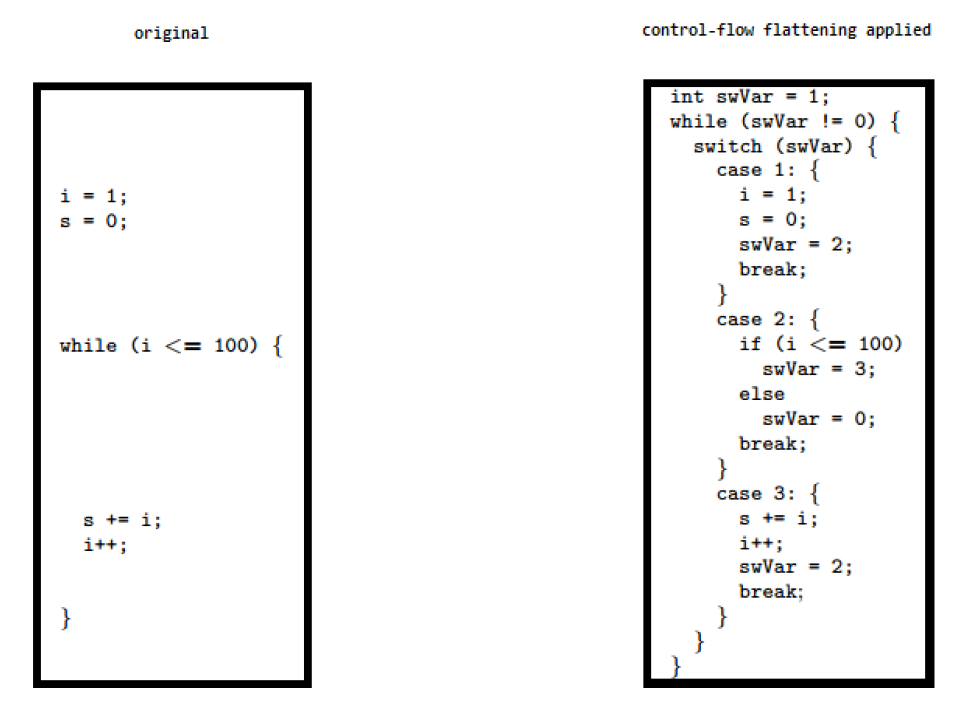
\includegraphics[width=0.8\textwidth]{./controlFlow.png}
    \captionsetup{labelformat=empty}
    \caption{Come il control-Flow altera il codice}
    \label{fig:cFlow}
\end{figure}


\newpage
\section{Reverse Engineering di InsecureShop}
InsecureShop\cite{insecureshop} è una applicazione Android scritta in Kotlin progettata per essere intenzionalmente vulnerabile. 
\`E un ottimo strumento per gli appassionati di sicurezza di Android poiché incorpora molte vulnerabilità.
Per poter effettuare questo esempio avremo bisogno dei seguenti strumenti:
\begin{enumerate}
    \item \textbf{InsecureShop}: il file APK\footnote{Formato delle applicazioni di Android} contenente l'applicazione mobile
    \item \textbf{Android Studio}: un IDE per lo sviluppo di Applicazioni Mobile per Android\cite{androidStudio} 
    comprensivo di un emulatore e in suo pacchetto di Strumenti SDK.
    \item \textbf{Platform Tools}: Pacchetto di Tools CLI\footnote{Command Line Input: comandi da usare in un terminale} 
    di Android; riguardo questo pacchetto, io ho riscontrato problemi poiché
    all'installazione il loro percorso non viene inserito nel PATH\footnote{PATH è una variabile di sistema utilizzata per 
    individuare più facilmente gli eseguibili} di Windows, potete inserilo voi li o potete fare come me, scaricare\cite{sdk} questo pacchetto, 
    inserirlo nella directory dove andremo ad operare sulle Mobile App ed 
    eseguirlo da una directory specifica aprendo il terminale lì\footnote{Premendo Maiuscola nella tastiera ed il tasto destro del mouse sulla cartella, vi apparirà 
    nel menù la scelta di aprire il prompt o PowerShell con il percorso della cartella.}.
    \item \textbf{Visual Studio Code}\cite{vscode}\textit{VSCode}, un editor della Microsoft che in realta è molto di più.
    \item \textbf{APKLab}:Estensione di VSCode scaricabile sia dal link citato qui\cite{apklab} o direttamente da VSCode cercandola nell'apposito 
    campo di ricerca nella sezione Estenzioni.Questa estenzione contiene in un unico pacchetto strumenti quali apktool\footnote{Usata per estrarre gli elementi all'interno 
    di APK in un formato non leggibile, vedi\cite{apktool}} e jadx\footnote{Dex to Java Decompiler: un tool che permette di convertire i file Android Dex 
    in codice sorgente Java\cite{jadx}} per abilitare funzionalità tra cui
    decompressione, decompilazione, patching del codice e riconfezionamento delle app direttamente dall'editor. 
\end{enumerate}
\newpage
\subsection{Avvio Emulatore e recupero prime informazioni App}
Per prima cosa avviamo l'Emulatore di Android Studio cosi da poter installare l'applicazione e iniziare a reperire informazioni iniziali. 
Dalla Schemata di Welcome clicchiamo "\textit{More Actions}" e da li "\textit{Virtual Device Manager}"
\begin{figure}[h]
  \centering
  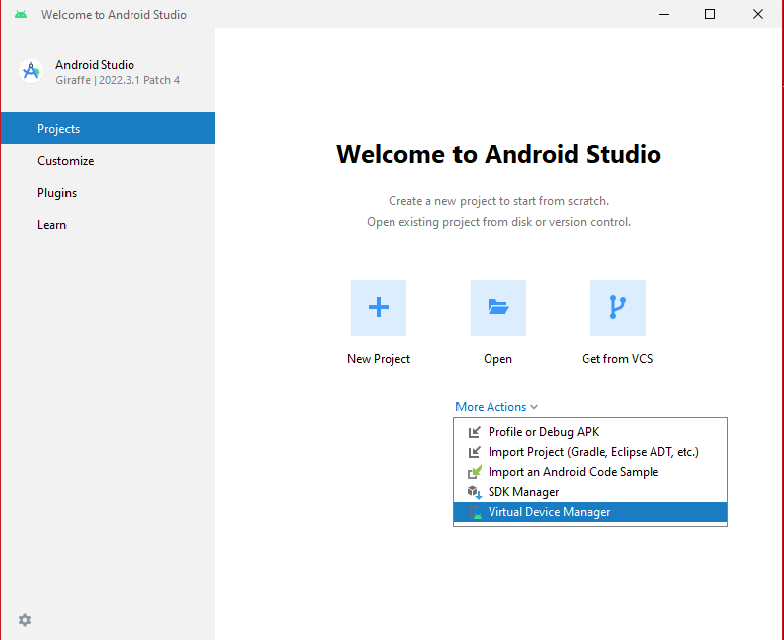
\includegraphics[width=0.5\textwidth]{./insecureshop/andStudDevice.png}
  \captionsetup{labelformat=empty}
  \caption{Avvio Virtual Device Manager}
  \label{fig:VDMStart}
\end{figure}

All'apertura della nuova finestra, dovrebbe già essere presente un emulatore\footnote{Se non dovesse essere presente, premere il pulsante 
"\textit{Create Device} per avviare la procedura guidata di creazione. Essa è molto intuitiva e facile sa eseguire"}, premete il simbolo play per 
iniziarne l'avvio: nel nostro caso emula un Pixel 3A con sistema Android 14.
\begin{figure}[h]
    \centering
    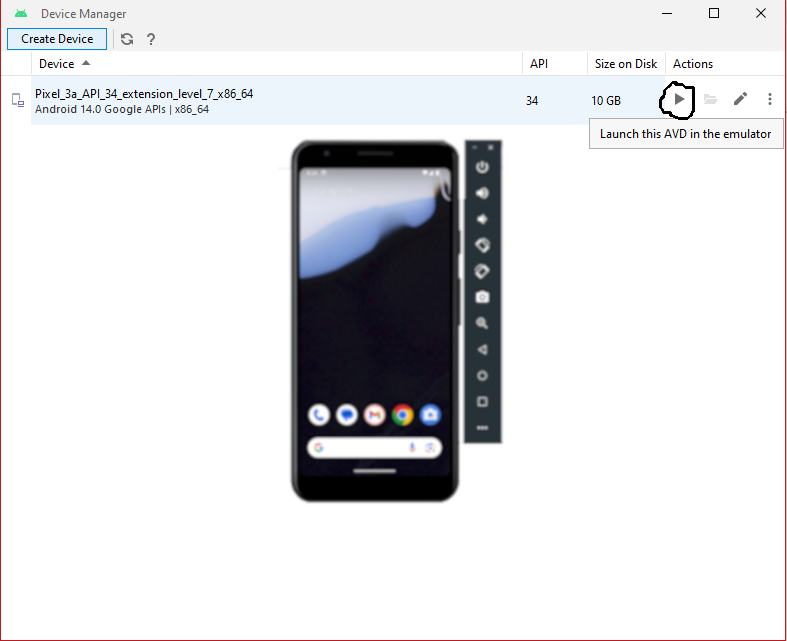
\includegraphics[width=0.5\textwidth]{./insecureshop/avvioADV.png}
    \captionsetup{labelformat=empty}
    \caption{AVD Avviato}
    \label{fig:avvioPhone}
\end{figure}

Adesso andiamo dove abbiamo salvato il nostro apk, preferibilmente una cartella dedicata, e utilizzando il tool adb.exe\footnote{Android Debug Bridge: strumento a riga di comando che ci permette di comunicare con nostro dispositivo Adroid} 
presente in Platform Tools\cite{sdk} di Android Studio installiamo la nostra App sul nostro emulatore scrivendo il seguente comando su
PowerShell e premendo invio:
\begin{verbatim}
    .\adb install ..\InsecureShop.apk
\end{verbatim}
Questo comando può essere usato tale e quale se il file InsecureShop.apk si trova nella cartella contenente anche la cartella Platform Tools
 che contiene adb.exe.
 \begin{figure}[htp]
    \centering
    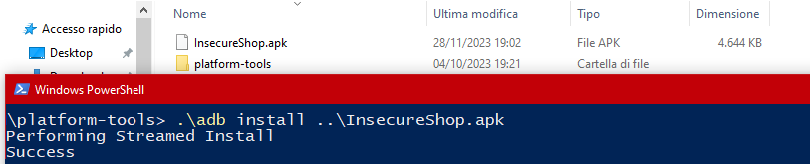
\includegraphics[width=0.8\textwidth]{./insecureshop/adbInstUse.png}
    \captionsetup{labelformat=empty}
    \caption{Installazione tramite adb.exe}
    \label{fig:installApp}
\end{figure}
\begin{figure}[htbp]
    \centering
    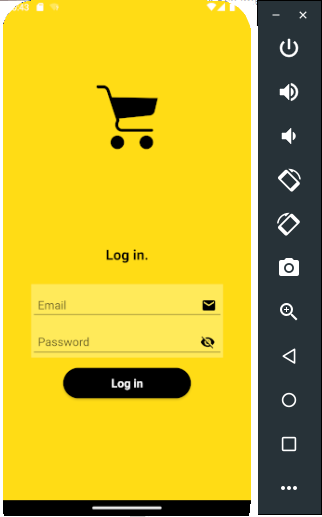
\includegraphics[width=0.30\textwidth]{./insecureshop/InsecureShopAvvio.png}
    \captionsetup{labelformat=empty}
    \caption{Applicazione InsecureShop all'avvio}
    \label{fig:InsecureShopStart}
\end{figure}

All'avvio dell'applicazione osserviamo essere presente una classica schermata di login con due spazi per Email e Password e un tasto con la 
dicitura "\textit{Log in}". Non essendoci altre informazioni ricavabili osservando, passiamo all'analisi del codice dell'applicazione.

\subsection{Estrazione Codice Sorgente}
Apriamo VSCode e eseguiamo la combinazione \textit{Ctrl+Shift+P} per aprire il riquadro dei comandi e digitare \textit{APKLab: Open an APK}.
Dalla schermata apertasi andiamo a trovare la cartella dove è stato salvato InsecureShop.apk e lo selezioniamo e premiamo \textit{OK}. 
Adesso APKLab aprirà una schermata su VSCode dove ci permetterà di selezionare delle opzioni aggiuntive:
selezioniamo \textit{"decompile\_java [use Jadx]"}, cosi indichiamo a APKLab di usare Jadx per decompilare i file dell'app, e diamo l'Ok.
\begin{figure}[t]
    \centering
    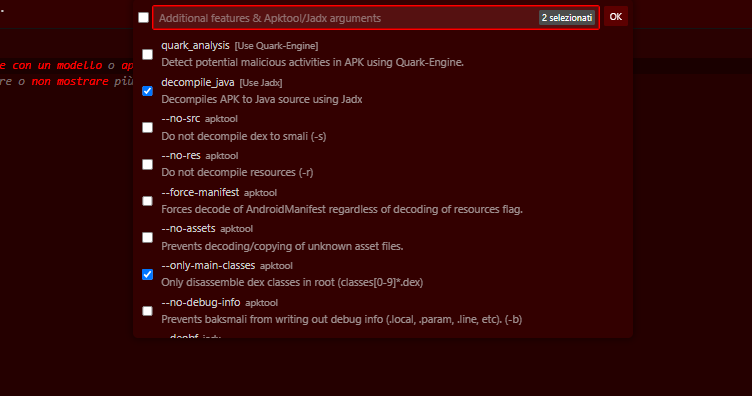
\includegraphics[width=0.8\textwidth]{./insecureshop/apklaboption.png}
    \captionsetup{labelformat=empty}
    \caption{Menù delle opzioni di APKLab}
    \label{fig:apklabOption}
\end{figure}

Dipende da quanto codice deve analizzare e convertire potrebbe richiedere qualche tempo per finire. Come possiamo vedere dalla figura \ref{fig:apklaboutput}
 Apklab utilizzerà due Tool:
\begin{itemize}
    \item Apktool: per decompilare l'applicazione e convertire i file in codice sorgente .dex
    \item Jadx: per decompilare i file .dex e convertirli in codice sorgente Java
\end{itemize}
Gli ultimi comandi, nella sezione \emph{Initializing}, sono dei comandi relativi a Git\footnote{Servizio per il salvataggio di
progetti in repository online} che non ha relazioni con il lavoro che dovremmo svolgere, possiamo anche eliminare la cartella .git generata.
\begin{figure}[hp]
    \centering
    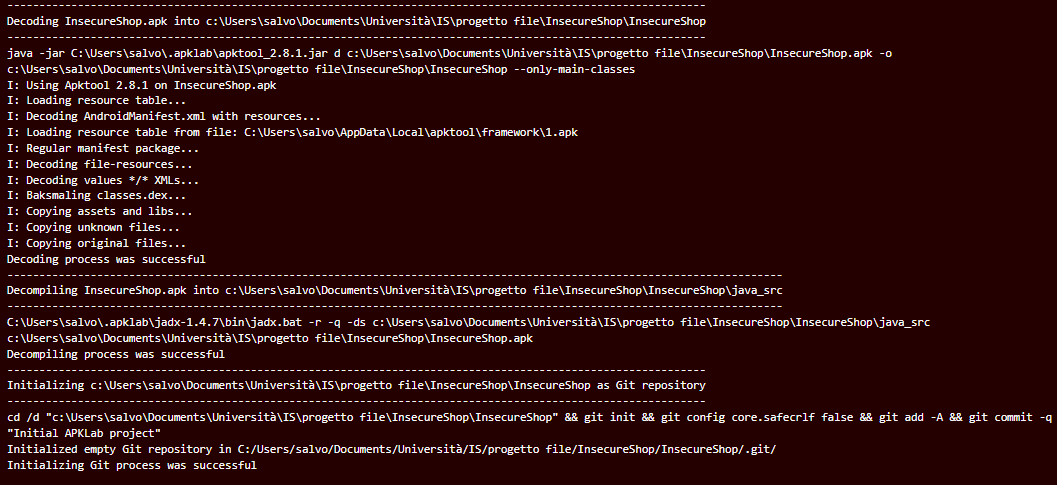
\includegraphics[width=1\textwidth]{./insecureshop/OutputApkLab.png}
    \captionsetup{labelformat=empty}
    \caption{Output APKLab}
    \label{fig:apklaboutput}
\end{figure}

\begin{figure}[htp]
\centering
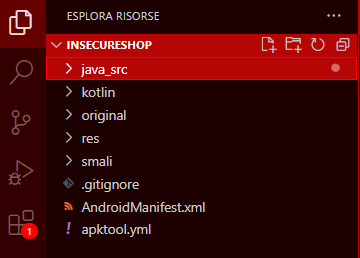
\includegraphics[width=0.5\textwidth]{./insecureshop/esploraRis.png}
\captionsetup{labelformat=empty}
\caption{Cartelle create da APKLab}
\label{fig:esplRis}
\end{figure}
\newpage
\subsection{Prima Analisi del Codice Estratto}
Andiamo su VSCode e per prima cosa andiamo a leggerci il file \emph{AndroidManifest.xml}, 
un file che fornisce importanti informazioni sulle caratteristiche dell'applicazione.
Per iniziare la nostra Analisi proviamo ad usare le informazioni che abbiamo: quando abbiamo avviato l'app 
ci siamo trovati di fronte ad una schermata di Log in,vediamo se c'è qualche cosa di correlato.

Su \emph{AndroidManifest.xml} troviamo una dicitura che cattura la nostra attenzione
\begin{verbatim}
    <activity android:name="com.insecureshop.LoginActivity"/>
\end{verbatim}
che ci indica che l'attività di Log in si trova in un file chiamato \textit{LoginActivity.java}.
Andiamo a cercare questo file, apriamo la cartella \textit{java\_src} e seguiamo il percorso \textit{com.insecureshop.LoginActivity}

Controllando il codice troviamo una funzione \textit{verifyUserNamePassword} usata per validare le credenziali d'accesso:

\begin{lstlisting}[style=JavaStyle]
boolean auth = Util.INSTANCE.verifyUserNamePassword(username, password);
if (auth) {
    Prefs prefs = Prefs.INSTANCE;
    Context applicationContext = getApplicationContext();
    Intrinsics.checkExpressionValueIsNotNull(applicationContext, "applicationContext");
    prefs.getInstance(applicationContext).setUsername(username);

    Prefs prefs2 = Prefs.INSTANCE;
    Context applicationContext2 = getApplicationContext();
    Intrinsics.checkExpressionValueIsNotNull(applicationContext2, "applicationContext");
    prefs2.getInstance(applicationContext2).setPassword(password);

    Util.saveProductList$default(Util.INSTANCE, this, null, 2, null);

    Intent intent = new Intent(this, ProductListActivity.class);
    startActivity(intent);

    return;
}
\end{lstlisting}

Questa funzione è chiamata da una Classe di nome Util importata all'inizio del file:

\begin{lstlisting}[style=JavaStyle]
import com.insecureshop.util.Util;
\end{lstlisting}

Andiamo a darle uno sguardo. Troviamo subito il metodo \emph{verifyUserNamePassword}:
\begin{lstlisting}[style=JavaStyle]
    public final boolean verifyUserNamePassword(String username, String password) {
        Intrinsics.checkParameterIsNotNull(username, "username");
        Intrinsics.checkParameterIsNotNull(password, "password");

        if (getUserCreds().containsKey(username)) {
            String passwordValue = getUserCreds().get(username);
            return StringsKt.equals$default(passwordValue, password, false, 2, null);
        }
        return false;
    }
\end{lstlisting}
In questo vediamo che viene usato un altro metodo \emph{getUserCreds} per controllare Username e Password:
\begin{lstlisting}[style=JavaStyle]
    private final HashMap<String, String> getUserCreds() {
        HashMap userCreds = new HashMap();
        userCreds.put("shopuser", "!ns3csh0p");
        return userCreds;
    }
\end{lstlisting}
L'Username e la Password sono codificate in chiaro in questa funzione, inseriamoli nell'applicazione.
\begin{figure}[htp]
    \centering
    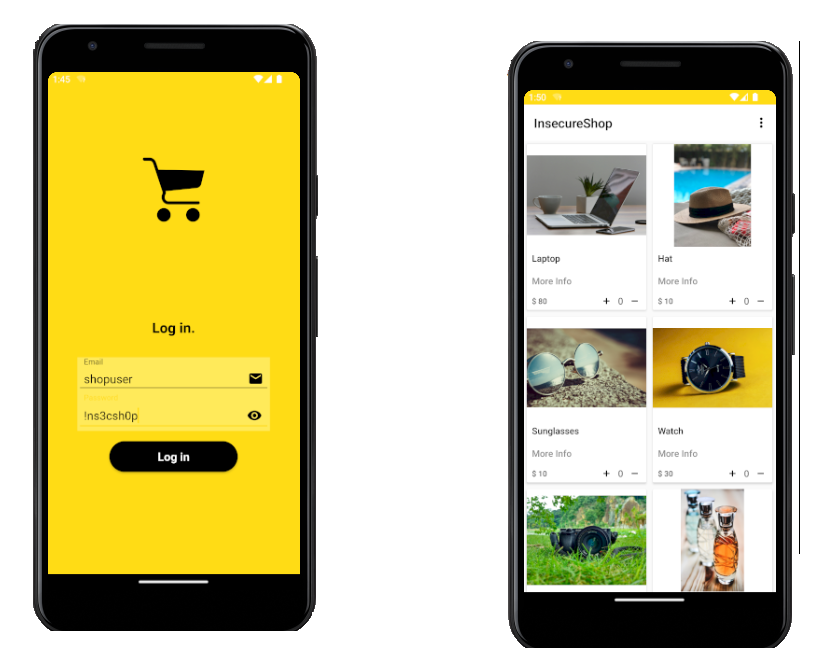
\includegraphics[width=0.5\textwidth]{./insecureshop/logIn.png}
    \captionsetup{labelformat=empty}
    \caption{Inserimento Credenziali trovate Nell'Applicazione}
    \label{fig:loginApp}
\end{figure}
Siamo riusciti a entrare!!!

Questo è un chiaro caso di \textit{Hardcoded Credentials}, di credenziali codificate direttamente nel codice. Questo tipologia 
di falla nella sicurezza affligge molti sistemi e continuerà a farlo perchè quando si pensa alla sicurezza nessuno pensa per prima 
cosa ad una password lasciata in chiaro, ma a cose ben più complicate finché non incappano in quel problema loro stessi. 

\subsubsection*{Contromisure}
Per poter evitare falle del genere si consiglia l'utilizzo del metodo di Obfuscation String Encryption, in modo da non rendere facile l'individuazione 
di credenziali ma anche di altre stringhe all'interno del codice. Si potrebbe
utilizzare una semplice funzione di crittografia come il Salt\footnote{ vedi Wikipedia \url{https://it.wikipedia.org/wiki/Salt_(crittografia)}} 
che prevede il salvataggio di una stringa ricavata dall'uso del metodo Salt e del Salt stesso per poter 
effettuare il confronto, questo renderebbe utilizzabili attacchi di tipo
BruteForce\footnote{Attacchi di forza bruta in cui si tenta di trovare la password in modo forzato provando le varie combinazioni}.
In alternativa, si potrebbero usare una \textbf{ Password tipo OTP}, \textit{One-Time Password}\footnote{Password utilizzabile solo una volta}, 
che, per la sua stessa natura, dopo 
l'accesso perde la loro funzione, così anche se salvate in chiaro sarebbero quasi inutilizzabili.
\subsection{Seconda Analisi del Codice}

Ritoniamo al nostro \emph{AndroidManifest.xml} e continuamo ad analizzare ciò che vi è scritto.
Sotto la riga di codice riferita al Login troviamo una segmento di codice che tratta la "Vista Web":
\begin{verbatim}
<activity android:name="com.insecureshop.WebViewActivity">
    <intent-filter>
        <action android:name="android.intent.action.VIEW"/>
        <category android:name="android.intent.category.DEFAULT"/>
        <category android:name="android.intent.category.BROWSABLE"/>
        <data 
            android:host="com.insecureshop" 
            android:scheme="insecureshop"/>
        </intent-filter>
</activity>  
\end{verbatim}
Ci segniamo il percorso all'interno della cartella java\_src della classe e andiamo a dare uno sguardo. La classe è collocata 
nel seguente percorso
\begin{verbatim}
    com.insecureshop.WebViewActivity.java
\end{verbatim}

Analizzando il codice ci imbattiamo in una falla nella sicurezza all'interno del metodo onCreate; in esso si controlla se 
all'interno del \textit{url} sono presenti le stinghe "\textit{/web}" o \textit{/webview} ma non controlla nessun altra cosa. 
Questo permetterebbe a chiunque voglia può costruirsi un suo URI e passare un parametro arbitrario come url; vediamo come possiamo farlo utilizzando 
adb Activity Manager e un URI:

\begin{verbatim}
.\adb shell am start -W -a 
   android.intent.action.VIEW -d 
   "insecureshop://com.insecureshop/web?url=
        https://en.wikipedia.org/wiki/Verification_and_validation"

   # am: activity Manager
   # start:Avvia una attività specificata da un Intent 
   # -W: aspetta la fine dell'avvio
   # -a: l'attività svolta dall'intent -d: intent URI 
\end{verbatim}
Quindi con questo comando avviamo una shell(terminale) nel nostro dispositivo android da cui avviamo un Activity Manager a cui diciamo di 
avviare uno specifico intent dato da intent URI che svolge una specifica attività, nel nostro caso "android.intent.action.VIEW" cioé di 
visualizzazzione.
\begin{figure}[htp]
    \centering
    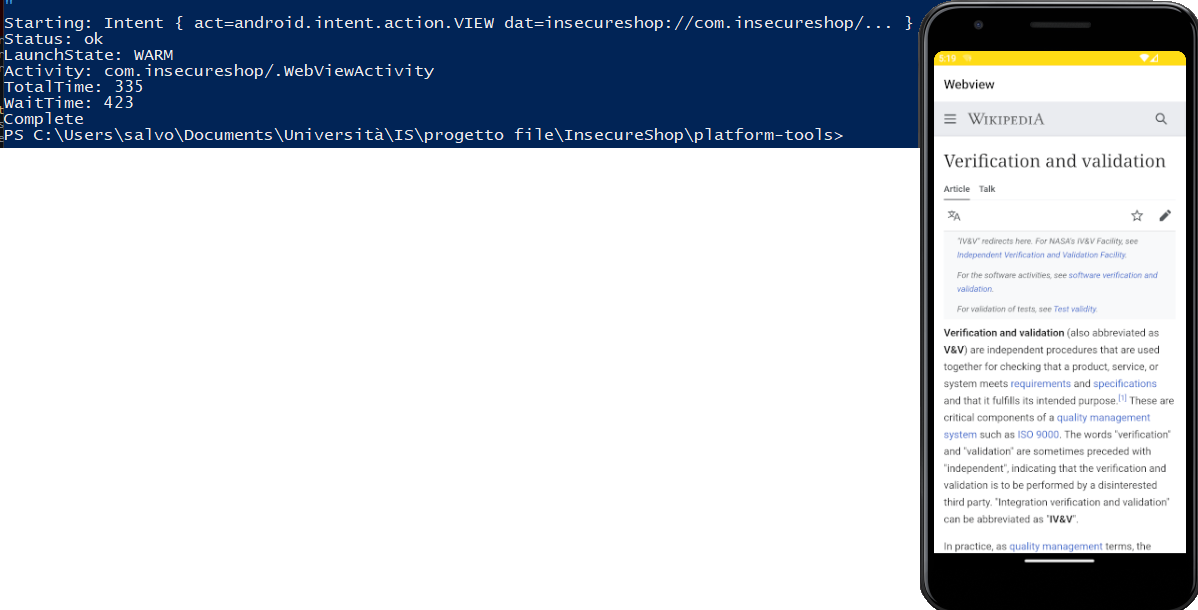
\includegraphics[width=0.8\textwidth]{./insecureshop/URIOutput.png}
    \captionsetup{labelformat=empty}
    \caption{Risultato del dell'invio di un URI intent alla nostra App}
    \label{fig:URIntent}
\end{figure}

\subsubsection*{Possibili Contromisure}
Per evitare questo problema Google chiede a tutti di associare all'applicazione un sito web su cui pubblicare un file JSON 
Digital Asset Links che indica le app associate al sito web e verificare gli intent dell'URL dell'app. Si possono associare 
più app ad un sito web e anche più siti ad una App. 

Se quindi si attiva la funzione \emph{android:autoVerify=true} e il dispositivo presenta un Android dal 6.0 in su, allora 
il sistema verificherà automaticamente gli host associati all'App.\cite{webAssoc}


\section{Reverse Engineering di UnCrackable1}
UnCrackable1\cite{uncrackable1} è una Applicazione messa a disposizione dalla OWASP per permettere a persone che hanno appena cominciato con 
il Reverse Engineering a muovere i primi passi. Vengono usati anche nel loro libro MASTG\cite{MASTG}.
Per poter efettuare questo esempio avremo bisogno:
\begin{itemize}
    \item \textbf{UnCrackable1.apk}: il file APK della OWASP contenente l'applicazione mobile;
    \item \textbf{Android Studio}\cite{androidStudio}: un IDE per lo sviluppo di Applicazioni Mobile per
    Android comprensivo di un emulatore e in suo pacchetto di Strumenti SDK;
    \item \textbf{Platform Tools}\cite{sdk}: Pacchetto di Tools CLI di Android; riguardo questo
    pacchetto, io ho riscontrato problemi poiché all’installazione il loro percorso non viene inserito nel PATH di Windows, potete inserilo voi li
    o potete fare come me, scaricare questo pacchetto, inserirlo nella directory dove andremo ad operare sulle Mobile App ed eseguirlo da una
    directory specifica, aprendo il terminale lì.
    \item \textbf{Visual Studio Code}\cite{vscode}: \textit{VS Code}, un editor della Microsoft che in realta è molto di più;
    \item \textbf{Apklab}\cite{apklab}: Estensione di VSCode scaricabile sia dal link citato qui\cite{apklab} o direttamente da VSCode cercandola nell'apposito 
    campo di ricerca nella sezione Estenzioni.Questa estenzione contiene in un unico pacchetto strumenti quali apktool\footnote{Usata per estrarre gli elementi all'interno 
    di APK in un formato non leggibile} e jadx\footnote{Dex to Java Decompiler: un tool che permette di convertire i file Android Dex 
    in codice sorgente Java\cite{jadx}} per abilitare funzionalità tra cui
    decompressione, decompilazione, patching del codice e riconfezionamento delle app direttamente dall'editor.
\end{itemize}


\subsection{Avvio Emulatore e recupero prime informazioni App}
Per prima cosa avviamo Android Studio e come abbiamo fatto prima, dalla schermata di Welcome clicchiamo "\textit{More Actions}" e da li 
"\textit{Virtual Device Manager}" 
\begin{figure}[htbp]
    \centering
    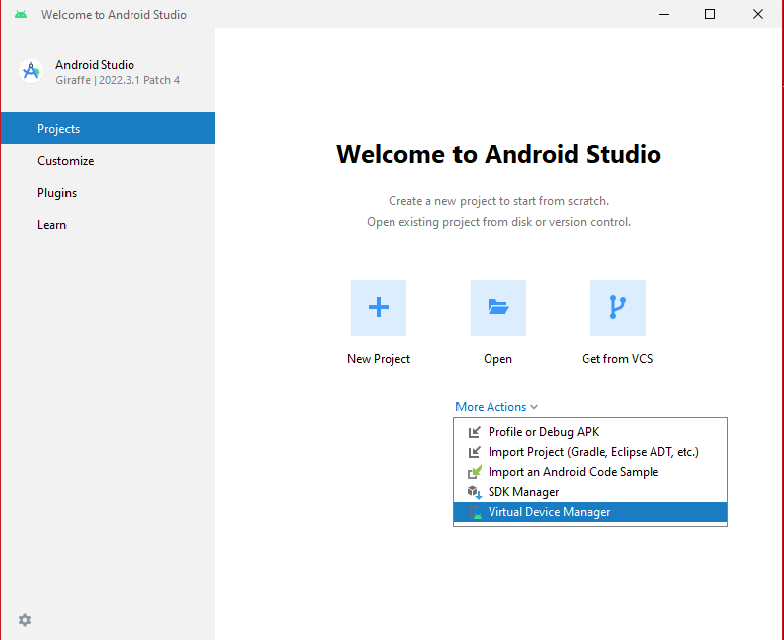
\includegraphics[width=0.6\textwidth]{./insecureshop/andStudDevice.png}
    \captionsetup{labelformat=empty}
    \caption{Avvio Virtual Device Manager}
    \label{fig:VDMStart2}
\end{figure}

All'apertura della schermata,cliccheremo il pulsante play del nostro emulatore e aspettando il suo avvio, andemo nella cartella 
dove abbiamo salvato UnCrackable1.apk insieme al SDK Platform Tools. 

Al suo avvio apriremo una PowerShell nella cartella di Platform e tramite adb.exe installeremo la nostra apk sul nostro dispositivo.
Ricordo cancora che il comando da usare è
\begin{verbatim}
    .\adb install ..\UnCrackable1.apk
\end{verbatim}

Finito il processo di installazione, andiamo ad aprire l'app. L'applicazione si presenta di grafica semplice: presenta solo 
una casella testuale e un tasto dalla dicitura \textit{VERIFY}. Provando ad inserire qualche cosa e cliccando Verify appare una 
messaggio che ci avvisa dell'inserimento della frase sbagliata.
Andiamo ad analizzare il codice.
\begin{figure}[htbp]
    \centering
    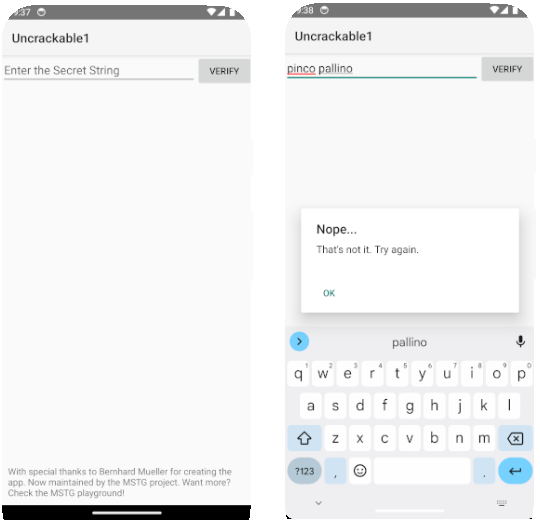
\includegraphics[width=0.5\textwidth]{./uncrackable1/avvioApp+Test.png}
    \captionsetup{labelformat=empty}
    \caption{Avvio e Analisi funzionamento App}
    \label{fig:AvvioTestApp}
\end{figure}
\newpage
\subsection{Estrazione Codice Sorgente}
Apriamo VS Code e eseguendo la combinazione \textit{Ctrl+Shift+P}, apriamo il riquadro di comandi e digitiamo 
\textit{Apklab: Open an APK}\footnote{Non è necessario scriverlo tutto, basta selezionarlo appena appare in lista}. 
Dalla schermata apertasi, andiamo a trovare la nostro app da analizzare e diamo OK, ricordiamoci di 
spuntare nel menù delle opzioni aggiuntive di APKLab il comando \textit{decompile\_java [use Jadx]}. 
\begin{figure}[htbp]
    \centering
    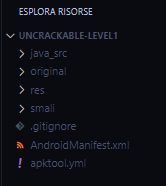
\includegraphics[width=0.3\textwidth]{./uncrackable1/apklabDirGen.png}
    \captionsetup{labelformat=empty}
    \caption{Directory Create da APKLab}
    \label{fig:apklabDirGen}
\end{figure}
In questo momento APKLab sta utilizzando due tools, Apktool\cite{apktool} e Jadx\cite{jadx} per decomprimere e ricompilare 
i sorgenti della nostra app in file leggibili per noi.

\subsection{Analisi del Codice Estratto}
Andiamo su VS Code e andiamo a dare un'occhiata al file \textit{AndroidManifest.xml}, un file che fornisce importati informazioni
 sulle caratteristiche dell'applicazione. L'unico riferimento presente all'interno dell'AndroidManifest.xml è 
 \begin{verbatim}
    <activity android:label="@string/app_name" 
          android:name="sg.vantagepoint.uncrackable1.MainActivity">
 \end{verbatim} 
 essa ci indica la classe principale \textit{MainActivity} che si trova al percorso \emph{sg.vantagepoint.uncrackable1.MainActivity}, 
 apriamola.
Ad una lettura della classe, individuiamo tre metodi: 
\begin{enumerate}
    \item \textit{a}.
    \item \textit{onCreate};
    \item \textit{verify};
\end{enumerate}

Il metodo \emph{OnCreate} è il primo metodo ad essere invocato all'avvio dell'applicazione che, salta subito all'occhio, contiene un metodo di 
riconoscimento per i \emph{Device Rooted}\footnote{il Rooting è un medoto che permette agli utenti di dispositivi android di ottenere controlli privilegiati
 sui vari sottosistemi Android, vedi \url{https://it.wikipedia.org/wiki/Rooting}} o che possono essere eseguiti in modalità \emph{Debaggable}\footnote{
Questo per evitare il debbugging che permette di vedere e modificare lo stato del software durante l'esecuzione}. Entrambi questi metodi ci mandano a controllare 
delle classi nel percorso \textit{sg.vantagepoint.a}. 

Questo metodo usa anche uno dei metodi presenti qui, \emph{a}, per riferire il messaggio 
del rilevamento del \textit{Root} o del \textit{Debug} attivo e aziona l'arresto immediato dell'applicazione alla conferma della visione del messaggio.
Il metodo \textit{verify} sembra sia correlato alla frase misteriosa da trovare, ci torneremo di sicuro dopo.

Anche se non ne avremmo bisogno pensiamo a come disattivare i metodi di controllo in \emph{onCreate}.
\subsubsection{Disabilitare Sistema Anti-Rooted}
Per prima cosa andiamo a controllare i metodi che permettono il riconoscimento dei sistemi con Root:
\begin{lstlisting}[style=JavaStyle]
    public static boolean a() {
        for (String str : System.getenv("PATH").split(":")) {
            if (new File(str, "su").exists()) {
                return true;
            }
        }
        return false;
    }

    public static boolean b() {
        String str = Build.TAGS;
        return str != null && str.contains("test-keys");
    }

    public static boolean c() {
        for (String str : new String[]{"/system/app/Superuser.apk", "/system/xbin/daemonsu", "/system/etc/init.d/99SuperSUDaemon", "/system/bin/.ext/.su", "/system/etc/.has_su_daemon", "/system/etc/.installed_su_daemon", "/dev/com.koushikdutta.superuser.daemon/"}) {
            if (new File(str).exists()) {
                return true;
            }
        }
        return false;
    }
\end{lstlisting}

Questi metodi controllano la presenza di determinate stringhe all'interno del OS Android per controllarne l'avvenuta modifica.

L'unico metodo per risolvere la situazione che sembra possibile effettuare è la modifica dei valori riportati dai vari metodi in 
modo che ritornino \textit{false} e, quindi, il recompilamento dell'applicazione.
Per fare ciò andiamo dal menù laterale sinistro ad aprire il corrispondente della classe \textit{MainActivity.java} all'interno delle classi 
generate in \emph{smali}.
\begin{figure}[htbp]
    \centering
    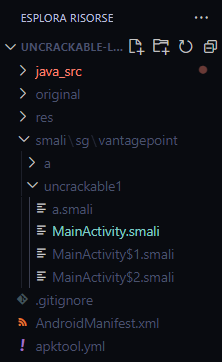
\includegraphics[width=0.3\textwidth]{./uncrackable1/smaliDir.png}
    \captionsetup{labelformat=empty}
    \caption{MainActivity all'interno della Directory Smali}
    \label{fig:smaliDir}
\end{figure}
%\newpage
Guardando i metodi scritti in smali, si decide per comodità di modificare non modificare tutti i metodi ma solo il metodo \emph{onCreate} 
cosi da non dover modificare troppo il codice.
\begin{figure}[h]
    \centering
    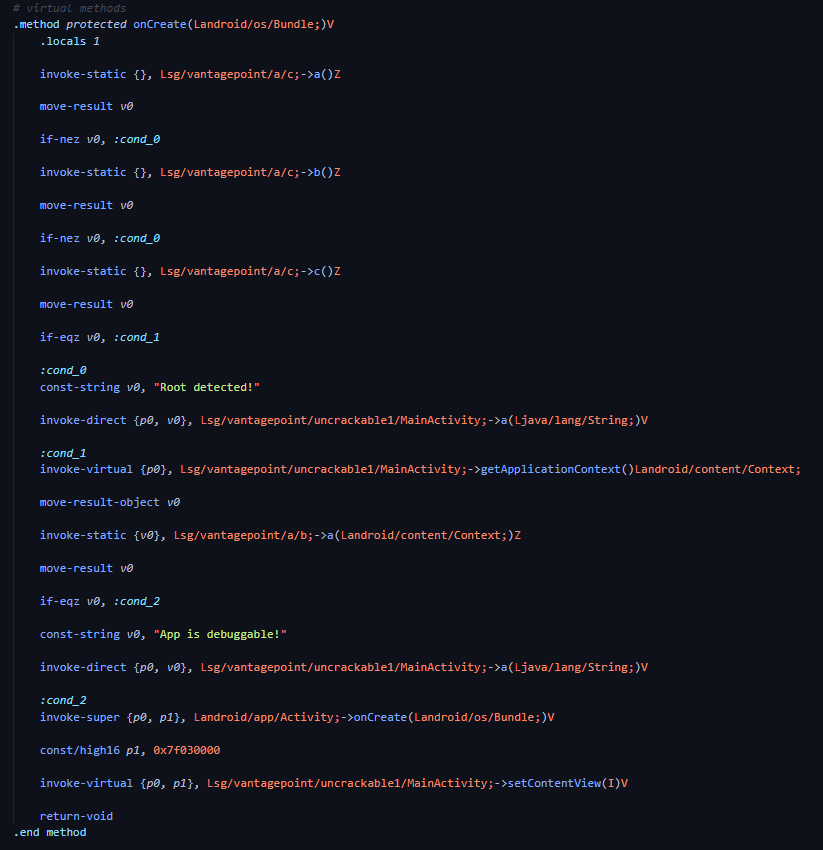
\includegraphics[width=0.75\textwidth]{./uncrackable1/OnCreateSmali.png}
    \captionsetup{labelformat=empty}
    \caption{Metodo onCreate nella Directory Smali}
    \label{fig:onCreateSmali}
\end{figure}

Prima di parlare delle modifiche da apportare diamo alcune semplici informazioni per poter interpretare questo codice smali:
Il seguente codice
\begin{verbatim}
    invoke-static {}, Lsg/vantagepoint/a/c;->a()Z
    move-result v0
\end{verbatim}
viene usato per invocare un metodo (\emph{invoke-static}), che non ha bisogno di parametri (\emph{\{\}})\footnote{quando si passa un parametro si scrive \{p0\}}
 facente 
parte della classe \textit{sq/vantagepoint/a/c} {\emph{Lsg/vantagepoint/a/c}}. Il nome del metodo invocato è a $( \rightarrow\emph{a}())$ che ritorna un 
booleano (\emph{Z}). Con \emph{move-result} si passa il valore ottenuto con il metodo alla variabile, in questo caso v0 che sarà 0 se viene ritornato false 
mentre 1 se è true.

I confronti fra due variabili vengono effettuati con la seguente codifica:
\begin{verbatim}
if-eq vA, vB, label   #valuta se vA e vB sono uguali.
if-ne vA, vB, label   #valuta se vA e vB non sono uguali.
if-eqz vA, label   #Valuta se vA è uguale a zero (FALSE).
if-nez vA, label   #Valuta se vA non è uguale a zero (TRUE).
\end{verbatim}
Il termine label qui usato fa riferimento ad una porzione del codice che inizia proprio col termite indicato in label,
il quale è il codice da eseguire se la condizione è verificata.

Per la dichiarazione di variabili, esse vengono indicate con la lettera v seguita da un numero e si dichiarano precedendole con il termine \emph{const}
\begin{verbatim}
const v0, 10 #Assegnamo il valore 10 a v0
const-string v0, "test" #equivale a String v0 = "test"
\end{verbatim}
Ad const di aggiungono elementi per specificare il tipo di da dichiarare, il registro e altro ancora.

Dopo aver dato questa introduzione al codice smali andiamo a modificare il testo. Come gia accennato prima io non andrei a modificare i 
metodi a, b, c, ma andrei a modificare l'azione effettuata da onCreate alla ricezione della conferma del Root o del Debug disponibile.

Quindi andremo a modificare i valori riportati dalle espressioni \textit{if-nez v0 :cond\_0} con \textit{if-nez v0 :cond\_1}. Qui trascrivo la spiegazione del codice:
\begin{verbatim}

    if-nez v0 :cond_0
    # Se v0 diverso da 0 esegui :cond_0 
    
    ...
    
    :cond_0
    const-string v0, "Root detected!"
    # String v0="Root detected!"
    
    invoke-direct {p0, v0}, 
        Lsg/vantagepoint/uncrackable1/MainActivity;
                                 ->a(Ljava/lang/String;)V
    # richiamo il metodo a(), 
    # percorso sg/vantagepoint/uncrackable1/MainActivity, 
    # passandogli il parametro, non ritorna nulla (Void)
    # Ricordo che il metodo a() in MainActivity è 
    #                                in metodo che chiude
    # l'app dopo che rileva delle anomalie

    :cond_1
    invoke-virtual {p0}, 
        Lsg/vantagepoint/uncrackable1/MainActivity;
            ->getApplicationContext()Landroid/content/Context;
    # Questo metodo va a richiamare una parametro 
    #                       che viene dato fornito da Android    
    
    move-result-object v0
    # passa il risultato del metodo precedente a v0

\end{verbatim}
Quindi diremo al sistema che se è Rooted, va a ricavare la variabile Context, cosi da evitare il richiamo al metodo a(), ma ancora non è finita.
Dobbiamo aggiungero una riga in modo da evitare la lettura della seguente parte di codice
\begin{verbatim}
    const-string v0, "App is debuggable!"

    invoke-direct {p0, v0}, 
        Lsg/vantagepoint/uncrackable1/MainActivity;
                                    ->a(Ljava/lang/String;)V
\end{verbatim}
Questo pezzo viene eseguito dopo \emph{if-eqz v0, :cond\_2} che si trova immediatamente dopo a \emph{:cond\_1} visto prima. 

Noi dobbiamo fare in modo 
che qualunque valore abbia v0 in questo \textit{if-eqz} il nostro codice vada a leggere \emph{cond\_2} dove si trova il metodo di avvio dell'app.
quindi aggiungimo sotto a \emph{if-eqz v0, :cond\_2} che anche se il valore non è zero si deve andare a leggere \emph{cond\_2}, per cui:

\begin{verbatim}
    if-eqz v0, :cond_2
    if-nez v0, :cond_2

    ...

    # ecco a voi anche il codice richiamato
    :cond_2
    invoke-super {p0, p1}, Landroid/app/Activity;
                            ->onCreate(Landroid/os/Bundle;)V
    # invoca la procedura di avvio 

    const/high16 p1, 0x7f030000
    # inizializza un paramentro, 
    # questo viene usato per i float in genere

    invoke-virtual {p0, p1}, 
        Lsg/vantagepoint/uncrackable1/MainActivity;
                                    ->setContentView(I)V
    # Questo ci carica gli elementi visivi
    
    return-void
    # riga finale di chiusura del metodo onCreate 
    # che ritorna Void cioé nulla
\end{verbatim}


Quindi per ricapitolare
\begin{itemize}
    \item cambiamo \emph{if-nez v0 :cond\_0}$\Rightarrow$  \emph{if-nez v0 :cond\_1}
    \item aggiungiamo\emph{if-nez v0, :cond\_2} sotto a \emph{if-eqz v0, :cond\_2}
\end{itemize}

Adesso dovremmo dare due cose: ricompilare UnCrackable1.apk con nostro codice modificato e avviarlo su un dispositivo Rooted
 per verificare che le correzioni funzionano. Ma visto che abbiamo gia tutto pronto continuiamo con la nostra analisi per trovare la 
 frase segreta.

\subsubsection{Ricerca Frase Segreta}
Ritorniamo a esaminare il file MainActivity.java e controlliamo il metodo \textit{verify()}:
\begin{lstlisting}[style=JavaStyle]
    public void verify(View view) {
        String str;
        String obj = ((EditText) findViewById(R.id.edit_text)).getText().toString();
        AlertDialog create = new AlertDialog.Builder(this).create();
        if (a.a(obj)) {
            create.setTitle("Success!");
            str = "This is the correct secret.";
        } else {
            create.setTitle("Nope...");
            str = "That's not it. Try again.";
        }
        create.setMessage(str);
        create.setButton(-3, "OK", new DialogInterface.OnClickListener() { 
            @Override 
            public void onClick(DialogInterface dialogInterface, int i) {
                dialogInterface.dismiss();
            }
        });
        create.show();
    }
\end{lstlisting}
Come possiamo vedere, esso crea una Stringa di nome \textit{obj} e le passa il testo scritto nella casella di testo dell'app. 
\textit{obj} viene
 passato come parametro al metodo
\textit{a()} che si trova in \emph{sg/vantagepoint/uncrackable1/a}, quindi nella stessa cartella di MainActivity.

Dato che questo metodo a() ritorna un 
boolean, sembra effettuare una qualche sorta di validazione, sembra che controllare questo metodo sia la strada giusta.
\begin{lstlisting}[style=JavaStyle]
public class a {
    public static boolean a(String str) {
        byte[] bArr;
        byte[] bArr2 = new byte[0];
        try {
            bArr = sg.vantagepoint.a.a.a(b("8d127684cbc37c17616d806cf50473cc"), Base64.decode("5UJiFctbmgbDoLXmpL12mkno8HT4Lv8dlat8FxR2GOc=", 0));
        } catch (Exception e) {
            Log.d("CodeCheck", "AES error:" + e.getMessage());
            bArr = bArr2;
        }
        return str.equals(new String(bArr));
    }

    public static byte[] b(String str) {
        int length = str.length();
        byte[] bArr = new byte[length / 2];
        for (int i = 0; i < length; i += 2) {
            bArr[i / 2] = (byte) ((Character.digit(str.charAt(i), 16) << 4) + Character.digit(str.charAt(i + 1), 16));
        }
        return bArr;
    }
}
\end{lstlisting}
Il metodo a() prende come input la frase che noi scriviamo nell'app e la confrota con la variabile bArr.\\ Se sono uguali il metodo ritorna TRUE, 
se non lo sono ritorna FALSE, per cui, in qualunque caso, la variabile \textit{bArr} contiene la frase in chiaro che stiamo cercando. 
Ora come facciamo a ottenerla?

Tutto ciò che serve alla generazione della Frase Segreta si trova qui, 
quindi se prendiamo tutto l'occorrente, possiamo dunque crearci una app che semplicemente calcoli la frase.

Andiamo su \textit{Android Studio} e cliccliamo \textit{New Project}. Nella schermata che appare selezioniamo rimaniamo sulla selezione \textit{Phone} nello specchietto 
a sinistra e a destra selezioniamo \textit{Empty View Activity}. Premiano \textit{Next}, in questa schermata cambiamo Language in \textit{Java}, cliccliamo \textit{Finish} e attendiamo la fine della creazione 
di questo progetto. Potrebbe volerci un pò per scaricare tutte le dipendenze, soprattutto se la vostra connessione non va molto veloce.
\begin{figure}[htbp]
    \centering
    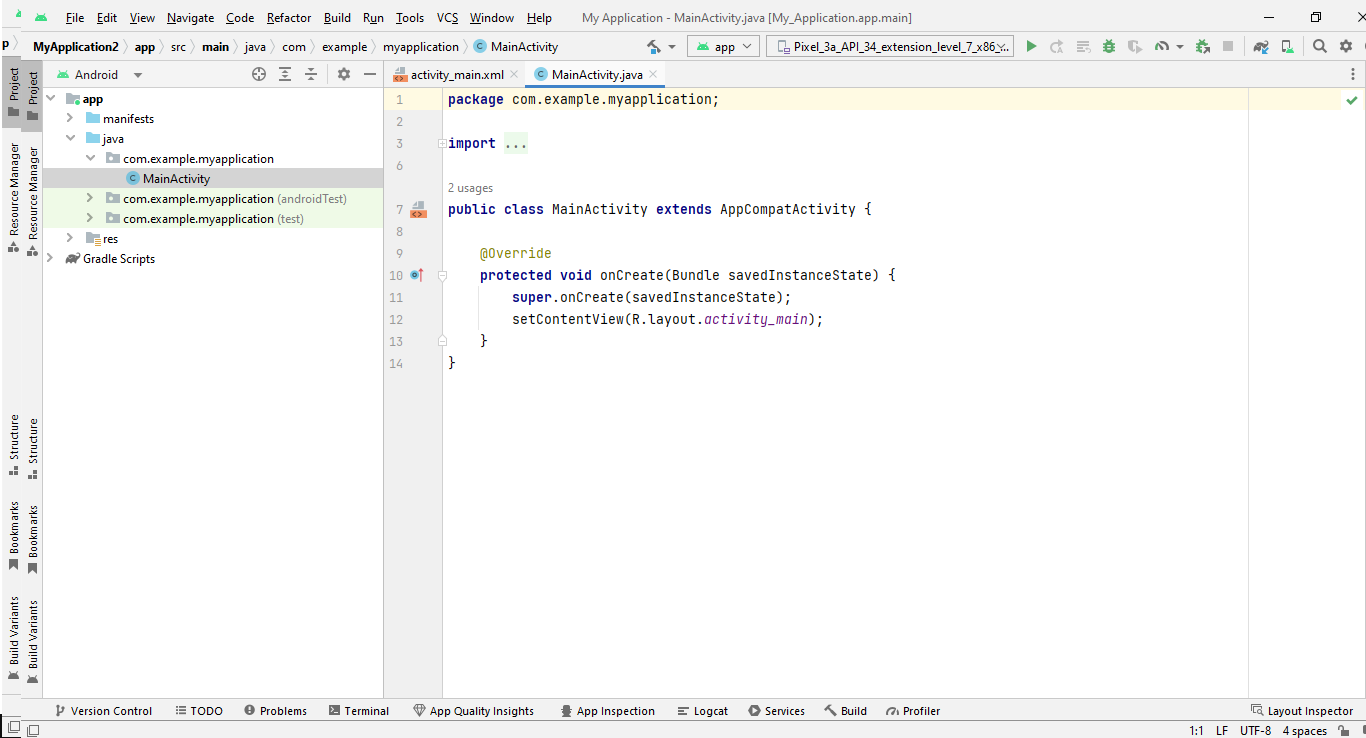
\includegraphics[width=0.8\textwidth]{./uncrackable1/appAndStud.png}
    \captionsetup{labelformat=empty}
    \caption{Nuovo Progetto con Android Studio}
    \label{fig:appAS}
\end{figure}

Appena finito il caricamento, iniziamo aggiungendo il codice dove è presente bArr nel metodo \textit{onCreate} della nostra nuova app,
 eliminado il riferimeto al percorso \emph{sg.vantagepoint.a.a} del rigo 6 e sostituendo al posto del \textit{return} (rigo 11) con
\begin{verbatim}
    Log.d("Solved", new String(bArr));
\end{verbatim}
per stampare su \textit{Logcat} la frase segreta. Ricorda di aggiungere il pacchetto del Log inserendo 
\begin{verbatim}
    import android.util.Log;
\end{verbatim}
all'inizio del file.

Al di fuori del metodo onCreate incolliamo i due metodi di supporto per il metodo appena inserito
\begin{lstlisting}[style=JavaStyle]
    public static byte[] b(String str) {
        int length = str.length();
        byte[] bArr = new byte[(length / 2)];
        for (int i = 0; i < length; i += 2) {
            bArr[i / 2] = (byte) ((Character.digit(str.charAt(i), 16) << 4) + Character.digit(str.charAt(i + 1), 16));
        }
        return bArr;
    }

    public static byte[] a(byte[] bArr, byte[] bArr2) {
        SecretKeySpec secretKeySpec = new SecretKeySpec(bArr, "AES/ECB/PKCS7Padding");
        Cipher instance = Cipher.getInstance("AES");
        instance.init(2, secretKeySpec);
        return instance.doFinal(bArr2);
    }
\end{lstlisting}


Se guardate il codice ci saranno dei metodi colorati in rosso, questo perché dobbiamo aggiungere gli import per Base64, Cipher e SecretKeySpec e indicare la gestione 
delle Eccezioni correlati a questi pacchetti. Per cui aggiungiamo
\begin{lstlisting}[style=JavaStyle]
import android.util.Base64;
import javax.crypto.Cipher;
import javax.crypto.spec.SecretKeySpec;

import java.security.InvalidKeyException;
import java.security.NoSuchAlgorithmException;

import javax.crypto.BadPaddingException;
import javax.crypto.IllegalBlockSizeException;
import javax.crypto.NoSuchPaddingException;
\end{lstlisting}

e  modifichiamo il metodo cosi:

\begin{lstlisting}[style=JavaStyle]
public static byte[] a(byte[] bArr, byte[] bArr2) throws InvalidKeyException, NoSuchPaddingException, NoSuchAlgorithmException, IllegalBlockSizeException, BadPaddingException {
    SecretKeySpec secretKeySpec = new SecretKeySpec(bArr, "AES/ECB/PKCS7Padding");
    Cipher instance = Cipher.getInstance("AES");
    instance.init(2, secretKeySpec);
    return instance.doFinal(bArr2);
}
\end{lstlisting}

Adesso non ci resta che eseguire l'applicazione cliccando il simbolo play verde in alto o premendo la combinazione "\textit{Shift+F10}\footnote{Shift è il tasto Maiuscola della tastiera}.
Aspettiamo la compilazione dell'app e l'installazione dell'app sull'emulatore, apriamo Logcat e nel campo di ricerca cerchiamo "\textit{Solved}".

Ecco trovata la Frase Segreta: \emph{I want to believe}.
\begin{figure}[htbp]
    \centering
    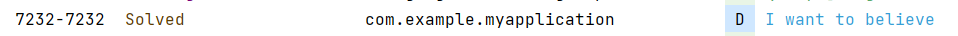
\includegraphics[width=1\textwidth]{./uncrackable1/soluzione.png}
    \captionsetup{labelformat=empty}
    \caption{Risultato Estratto da Logcat}
    \label{fig:logSol}
\end{figure}

Adesso per finire non ci resta che provare la frase ma per fare ciò dobbiamo avere a disposizione in nostro apk modificato per eliminate Anti-Root e 
un dispositivo dove verificare se la nostra modific funzioni.


\subsubsection{Creazione Device Rooted on Android Studio e Build Apk modificato}
Per ricompilarlo basta cliccare col tasto destro del mouse sul file \textit{apktool.yml} presente su "\textit{Esplora Risorse}" nella parte 
sinistra di VS Code e selezionare \textit{APKLab: Rebuild the APK}, alla comparsa del menu a tendina deselezioniamo "\textit{--use-aapt2}" poiché la nostra 
app non usa questo pacchetto per la generazione del suo codice binario ma \textit{aapt}.
\begin{figure}[htbp]
    \centering
    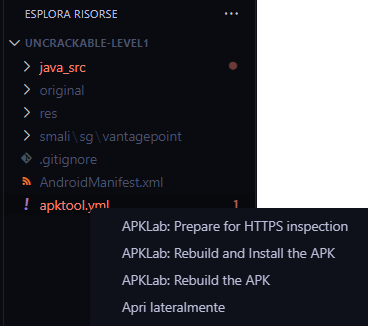
\includegraphics[width=0.4\textwidth]{./uncrackable1/rebuild.png}
    \captionsetup{labelformat=empty}
    \caption{APKLab: Rebuild The APK}
    \label{fig:rebuildApk}
\end{figure}

Uno dei motivi per cui ho deciso di utilizzare APKLab è perchè racchiude in se molti tools utili e uno di questi viene usato proprio in questo momento: \textbf{APKSigner}.

\textit{Apksigner} ci permette di inserire una firma alla nostra applicazione senza la quale i dispositivi android non vorranno eseguirla. Questa firma non è una forma di blocco 
dell'esecuzione dell'app, ma più una forma di protezione per l'inserimento dell'app da parte di terzi all'interno dello Store. 
Essa fa riferimento ad un Certificato dell'azienda creatrice o del creatore dell'apk. 
Quindi, identifica il proprietario dell'Applicazione Mobile e permette il ridiuto dell'applicazione nel caso in cui, al momento del caricamento di 
una nuova versione, essa non corrisponda con quella memorizzata. Il sistema usato per queste firme è quello della crittografia Asincrona. 

Nel nostro caso non ci vogliamo spacciare per nessuno, ma vogliamo solo permettere all'applicazione di essere eseguita senza problemi. L'Apk generato 
verrà salvato all'interno della cartella dist del progetto dell'apk decompilato, che si trova nella stessa cartella del unCrackable1.apk iniziale.

Adesso che abbiamo l'applicazione modificata da noi in formato apk, torniamo su Android Studio e, visto che adesso abbiamo un progetto in lista, per 
andare su \textit{Visual Device Manager}, dobbiamo premere i tre puntini in alto a destra e selezionare Visual Device Manager.
\begin{figure}[htbp]
    \centering
    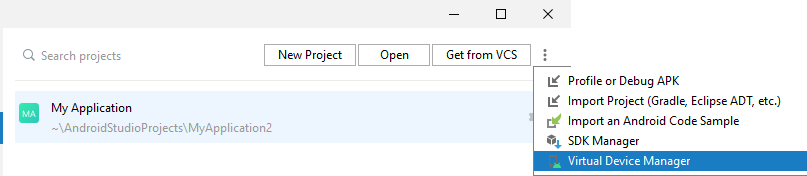
\includegraphics[width=0.8\textwidth]{./uncrackable1/NewDev.png}
    \captionsetup{labelformat=empty}
    \caption{Accede a Visual Device Manager dalla lista Progetti}
    \label{fig:vdmNew}
\end{figure}

All'apertura della seconda pagina contenete le Device, cliccate in alto a sinistra "\textit{Create Device}" e attendiamo l'apertura della procedura 
guidata per la creazione della nuova Device. Lasciamo la scelta su Phone in "\textit{Category}", dalla lista accanto scegliamo un modello di Smartphone,
 io ne consiglio uno con una schermo largo cosi da poter vedere meglio. Nel mio caso ho scelto un \textit{Pixel 4 XL} da 6.3".

Clicchiamo Next e adesso ci tocca scegliere l'OS Android da usare. Per il nostro bisogno passiamo alla schermata con scritto \textit{x86 Images} e scegliamone uno 
dalla lista. Io ho scelto il sistema Tiramisù con API 33 e Android 13, cliccando Next se non avete mai scaricato quella Image, iniziera il suo download.
Adesso vi apparirà una schermata di riepilogo in cui io ne ho approfittato per inserire la parola "ROOTED" in AVD Name cosi da poterlo distinguere dagli altri 
se dovessi avere più Device uguali. Clicchiamo Finish.
\begin{figure}[htbp]
    \centering
    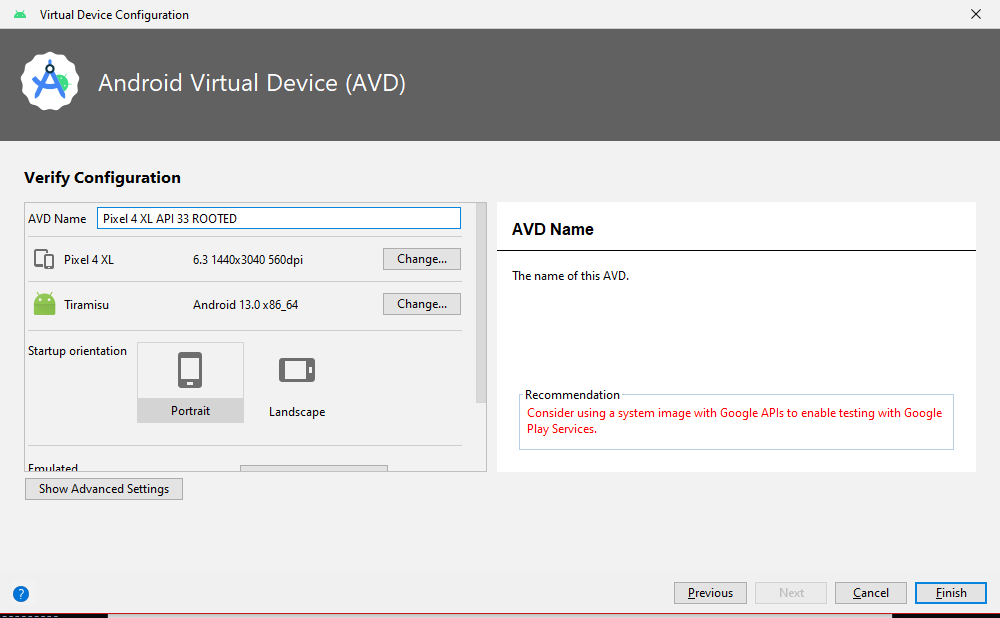
\includegraphics[width=0.8\textwidth]{./uncrackable1/Tiramisu.png}
    \captionsetup{labelformat=empty}
    \caption{Riepilogo creazione Device con Root}
    \label{fig:AVDRoot}
\end{figure}
\newpage
Avviamo il nuovo emulatore e per prima cosa installiamo la nostra App iniziale come test per il controllo del Root.

\begin{figure}[h]
    \centering
    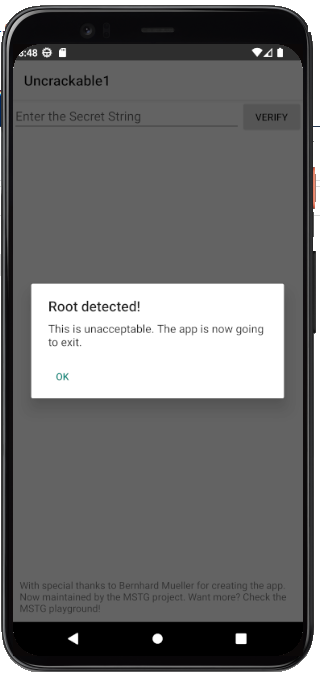
\includegraphics[width=0.25\textwidth]{./uncrackable1/primoTestRoot.png}
    \caption{Blocco applicazione per Device Rooted}
    \label{fig:rooted}
\end{figure}
Come si vede nella Figure\ref*{fig:rooted} l'applicazione riconosce il dispositivo come Rooted. Disinstalliamo questa app e tramite il comando 
\begin{verbatim}
 .\adb install ..\UnCrackable-Level1\dist\UnCrackable-Level1.apk
\end{verbatim}

installiamo la nostra applicazione modificata e essa si avvia senza problemi, adesso inseriamo la Frase Segreta trovata in precedenza ( I want to believe).
Siamo riusciti nel nostro intento. 

\begin{figure}[h]
    \centering
    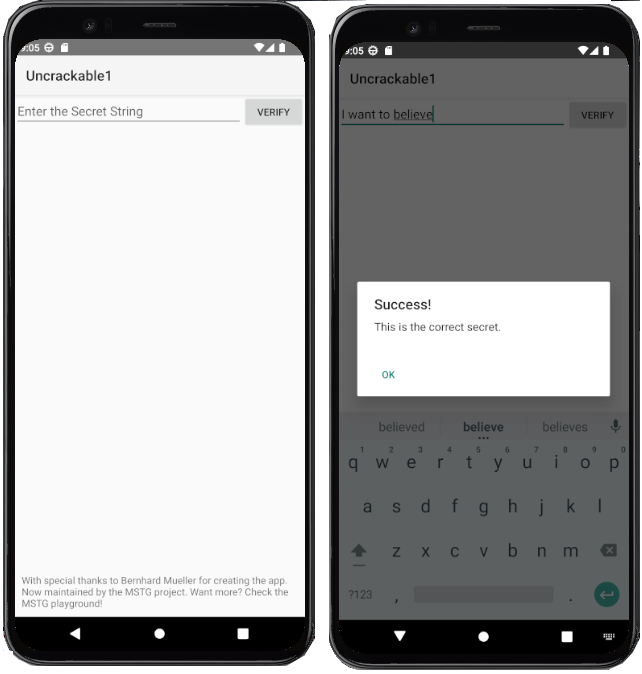
\includegraphics[width=0.45\textwidth]{./uncrackable1/modded.png}
    \captionsetup{labelformat=empty}
    \caption{Apertura applicazione modificata senza avviso e inserimento frase}
    \label{fig:modded}
\end{figure}


\subsubsection*{Contromisure}
In questo apk è stato applicato solo il minimo necessario di tecniche di Obfuscation e protezione. L'unica contromisura per la prevensione sarebbe l'aumento di sicurezza per proteggere il metodo 
di recupero della frase e di utilizzare 
più tecniche di Obfuscation come lo String Encryption, Dead Code Injection, la sostituzione delle istruzioni e aumentare il livello del Name Obfuscation 
usato.






\newpage
\section{Conclusioni}
Scrivere questa relazione non è stato facile. Non è stato facile trovare Applicazioni Mobili sullo Store su cui preparare questo testo perché tutte superavano 
la mia preparazione. Pur avendo appreso 
il funzionamento generico e l'uso dei strumenti usati in questa relazione,il Reverse Engineering di tali applicazioni richiederebbe conoscenze specifiche che io non possiedo. 

Per questo mi sono affidato ad 
applicazioni create per questo scopo. Mi è stato impossibile poter fornire un esempio di Reverse Engineering Mobile su sistemi iOS perché 
non ho potuto trovare gratuitamente un Emulatore iOS adatto e le alternative trovate richiedevano il possesso di un dispositivo fisico della Apple.

Comunque abbiamo parlato delle basi per effettuare un Reverse Engineering sulle applicazioni, di come è possibile effettuarlo, visto degli esempi,  
di come può essere utile per la sicurezza e per l'analisi dei malware e delle tecniche di prevenzione.
\medskip

Essere capace di effettuare un Reverse Engineering su un'applicazione e capire, per modificare o altro,
il suo funzionamento interno è un grade "superpotere" da avere, ma che richiede grande impegno e dedizione poiché, come affermato anche da OWASP, 
su questo argomento si possono riempire librerie intere e io so di aver visto solo la punta dell'Iceberg.

Alla fine posso dire, nel mio piccolo, di essere d'accordo con OWASP:\\ \textit{il Reverse Engineering è un'arte}. 
\begin{thebibliography}{9}
    %\bibitem{RE.ethics.csc.ncsu.edu} \textit{"Reverse Engineering"}, ethics.csc.ncsu.edu link:\url{https://ethics.csc.ncsu.edu/intellectual/reverse/study.php}
    \bibitem{REWikipedia} Wikipedia. \textit{Reverse Engineering} \url{https://en.wikipedia.org/wiki/Reverse_engineering}
    \bibitem{AWiki} Wikipedia. \textit{Applicazione Web} \url{https://it.wikipedia.org/wiki/Applicazione_web}
    \bibitem{MASTG} OWASP, Ottobre 2023. \textit{Mobile Application Security Testing Guide (MASTG) v1.7.0}.  Disponibile su \url{https://mas.owasp.org/MASTG/}
    \bibitem{MASVS} OWASP. \textit{Mobile Application Security Verification Standard (MASVS)} Disponibile su \url{https://mas.owasp.org/MASVS/}
    \bibitem{reDef} TechTarget. \textit{Reverse Engineering} \url{https://www.techtarget.com/searchsoftwarequality/definition/reverse-engineering}
    \bibitem{owasp2016} OWASP. 2016. \textit{Mobile Top 10}. Estratto da \url{https://owasp.org/www-project-mobile-top-10/2016-risks/}
    \bibitem{owasp2023} OWASP. \textit{Mobile Top 10}. Estratto da \url{https://owasp.org/www-project-mobile-top-10/}
    \bibitem{Assembly} Wikipedia. \textit{Assembly Language} \url{https://en.wikipedia.org/wiki/Assembly_language}
    \bibitem{smali} Just Mobile Security, Luglio 2023. \textit{Android Static Analysis Fundamentals: Smali Code Introduction and Modifications}. LinkedIn \url{https://www.linkedin.com/pulse/android-static-analysis-fundamentals-smali-code-introduction}
    \bibitem{webAssoc} Android developers. \textit{Verifica i Link per app Android} \url{https://developer.android.com/training/app-links/verify-android-applinks?hl=it#web-assoc}
    \bibitem{firmDigAtlas} Istituto Italiano Edizioni Atlas. \textit{Firma dell'app e pubblicazione nello Store} \url{https://www.edatlas.it/scarica/Informatica/prosia_5_2019/Capitolo5Mobile/MaterialiOnline/FirmaPubblicazioneApp.pdf}
    \section*{Applications \& Tools}
    \bibitem{androidStudio} Android Studio IDE. \url{https://developer.android.com/studio}
    \bibitem{sdk} SDK Platform Tools. \url{https://developer.android.com/tools/releases/platform-tools}
    \bibitem{vscode} Visual Studio Code, Windows \url{https://code.visualstudio.com/}
    \bibitem{apklab} Surendrajat. \textit{APKLab}, VSCode. \url{https://marketplace.visualstudio.com/items?itemName=Surendrajat.apklab}
    \bibitem{apktool} Apktool, Android. \url{https://github.com/iBotPeaches/Apktool}
    \bibitem{jadx} Jadx, Android \url{https://github.com/skylot/jadx}
    \bibitem{insecureshop} InsecureShop.apk , Android. \url{https://github.com/hax0rgb/InsecureShop}
    \bibitem{uncrackable1} MAS Crackmes. \url{https://mas.owasp.org/crackmes/}
    \bibitem{frida} Frida. Dynamic Instrumentation Toolkit \url{https://frida.re/}
    \bibitem{wireshark} WireShark \url{https://www.wireshark.org/}
\end{thebibliography}

\end{document}
